\vspace*{1ex}

\section{Introduction}

\noindent As moving to a new age, people tend to need more communication. Filling the gap between different cultures requires translating countless books, articles and words. Human resource is always a limitation. Thousands of 
pioneers have developed a serious of Mathematical model for doing translation mechanically. 

Much of the previous model employ too much mathematics,
	focus not enough to the true meaning of the words.
Translate is not a simple mapping from source language to target language.
In order to do perfect translation,the true meaning of the words must be understood. 

Making a computer program understand a string is the so called
	 \hbox{\emph{Lexical}} 	\hbox{\emph{Analyse}}. 
When Lexical Analyse finished, the given string will be converted into a abstract syntax tree. 
This tree represents the internal meaning and structure of the analysed string.
Since it's a data struct, programs will find it more easier to do further analyse.
\nocite{Compilers_Principles_Techniques_and_Tools}


Before doing the Lexical Analyse, the string should be tokenized and the every token should be marked by it's part of speech.
This process is called, syntax analyse.

\section{Body}

\subsection{Tokenize}
Before doing any other thing, a subsequence of text need to be divided into tokens\footnote{You can consider tokens as words, but tokens is far more than just words.\footnotemark}.
\footnotetext{Punctuations are also tokens.}
A token is an unbreakable group of symbols.

Tokenize can be performed by regular expression. In English, tokens are separated by spaces.
Lex\cite{Lex} helps write programs whose control flow is directed by instances of regular expressions in the input stream. Lex source is a table of regular expressions and corresponding program fragments. The table is translated to a program which reads an input stream, copying it to an output stream and partitioning the input into strings which match the given expressions. As each such string is recognized the corresponding program fragment is executed. The recognition of the expressions is performed by a deterministic finite automaton generated by Lex. The program fragments written by the user are executed in the order in which the corresponding regular expressions occur in the input stream. Lex has a very up to date drop in replacement: Flex\cite{flex}. 

\subsection{Part-of-speech Tagging}

After tokenization, there comes part-of-speech tagging.

Let's consider this input :
\framedparbox{
The Fulton County Grand Jury said Friday an investigation of Atlanta's recent primary election produced "no evidence" that any irregularities took place.
}\\\indent
and tagging every words like this:
\framedparbox{
The/at-tl Fulton/np-tl County/nn-tl Grand/jj-tl Jury/nn-tl said/vbd Friday/nr an/at investigation/nn of/in Atlanta's/np\$ recent/jj primary/jj election/nn produced/vbn "/" no/at evidence/nn "/" that/cs any/dti irregularities/nns took/vbd place/nn ./.
}

Tagging a text first require you to have a tag set\footnote{Kinds of token.}.
 Brown Corpus
% \footnote{参考\url{http://clwww.essex.ac.uk/w3c/corpus_ling/content/corpora/list/private/brown/brown.html}.}
 defines 87 tag set. For machine translation, a smaller set will be enough. 
 
For English ,  I put some definitions that will be used next:
\begin{enumerate}

\item We have a huge set $W$ that contains every English word on earth.

\item For $ \lambda_n \in w_1 , w_2 , w_3, \ldots , w_{i-1} , w_i  , \ldots , w_m \in W $ , they
		form a sentence $Wr$. $m$ is the length of the sentence $Wr$ 
\item We assign every word one or more part-of-speech, and use one integer representing  one type of part-of-speech, also, punctuations also got it's value. Then we got  a  small set that have every integer represent one type of words or punctuations (or token I will call them subsequently ), we call this set $ P $.
\item For a given sentence $Wr$, every word will got only one part-of-speech due to the context.
We let $W_i \in W $ represent the i\textsuperscript{th} token, then $ \, Wr = w_1 + w_2 + w_3 + \ldots + w_{i-1} + w_i  + \ldots + w_m  \, $ , since every token can have only one type regardless the fact that the same token will have different type in other sentence (or context), we let $P_i \in P $ represent the type of i\textsuperscript{th} token, then we got $Pr$ , aka $ Pr = p_1 + p_2 + p_3 + \ldots + p_{i-1} + p_i + \ldots + P_m $. 

\item $Pr $ and $ Wr $ have the same item count and same item sequence. $ W_i$ is mapped to $ P_i $. We use formula $ Pr = WP(Wr)$ to stand for this mapping. % $ Pr=\sum_{i=1}^{m} P_i  , P_i \in P , Wr=\sum_{i=1}^{m}W_i, W_i \in W$  
\end{enumerate}

This mapping can be done by ANN\footnote{Artificial neural network, see \url{http://www.learnartificialneuralnetworks.com/} for more details. }.
ANN is a function between very very complex input and output such as the function that get a photo as input, print name of the people inside the photo as output \footnote{Yes, it's called Face-recognition}.

Before processing, $P_i$ can have many but limited ( $\in P$) possible  assignment. The number of the possible assignment is $[1, \#P ] $ , let mark it $ C_i $. 
And if there is a dictionary\footnote{Mostly, the words' part-of-speech can be done by a simple lookup in the dictionary.}, $ C_i $ most possible value will $ \equiv 1 $. 

The tagging task, we need to find the exact value of $P_i$ for $W_i$, and each $P_i$ can be value $ \in P $ ,  each value have it's own \emph{probability} can the probability can be reflected by $ W_i \in Wr $ . So, what's the best suitable ANN for this kinds of task? Yes, it's HMM\footnote{Hidden Markov model}{\citep{HMM_Based_Part_Of_Speech_Tagging}}.

HMM is first introduced by \emph{Leonard E. Baum} in a series of statistical papers in the second half of the 1960s. Later on, people developed a great kinds of part-of-speech tagging based on HMM algorithm. 

In HMM, $ Wr $ can be viewed as \emph{Observation symbols}, so $Pr$ is \emph{Hidden symbols}. Dictionary can helped, but some time when dictionay can't help, HMM's ``learn'' ability  can be used. As I mentioned, HMM is kind of an ANN, so HMM inherited ``learning'' ability from ANN.
HMM can learned to calculate the most possible value of very $P_i$. Thus, the tagging is achieved

\subsection{Concrete Syntax Tree Generating}

A concrete syntax tree\cite{cst} or parse tree is an (ordered, rooted) tree that \mbox{represents} the syntactic structure of a string according to some formal grammar.
\begin{wrapfigure}{}{13em}
\begin{center}
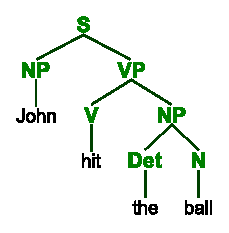
\includegraphics{../ParseTree}
\caption{A simple parse tree}
\end{center}
\end{wrapfigure}
In a parse tree, the interior nodes are labeled by non-terminals of the grammar, while the leaf nodes are labeled by terminals of the grammar. Parse trees may be generated for sentences in {\em \mbox{natural} \mbox{languages}},  as well as during processing of computer languages, such as programming languages. Parse trees are \mbox{distinct} from abstract syntax trees (also known \mbox{simply} as syntax trees), in that their structure and \mbox{elements} more concretely reflect the syntax of the \mbox{input} language.

Syntax tree  can be descriped in BNF\footnote{Backus–Naur Form}.
BNF\cite{BNF} is a notation technique for context-free grammars, often used to describe the syntax of languages used in computing, such as computer programming languages, document formats, instruction sets and communication protocols. It is applied wherever exact descriptions of languages are needed, for instance, in official language specifications, in manuals, and in textbooks on programming language theory.

A BNF specification is a set of derivation rules, written as
\framedparbox{
\vspace*{2ex}
 <symbol> ::= \_\_expression\_\_ 
\vspace*{2ex}
 }

where <symbol> is a nonterminal, and the \_\_expression\_\_ consists of one or more sequences of symbols; more sequences are separated by the vertical bar, `|' , indicating a choice, the whole being a possible substitution for the symbol on the left. Symbols that never appear on a left side are terminals. On the other hand, symbols that appear on a left side are non-terminals and are always enclosed between the pair <>.

Let's see the example BNF that described \fbox{\texttt{John hit the ball}} 
\framedparbox{
\vspace*{2ex}
ENDPUNC ::= '.' | '?' 

S ::= NP VP ENDPUNC | NP ENDPUNC | VP ENDPUNC | ...  < more >

NP ::= Det N | N  | Pron | < more >

Det ::= "the" | "an" | "a" | "this" | ... ...  < more >

V ::= "hit" | ...... < more >

N ::= "ball" | .... < more >

Pron ::= I | "you" | ..... <more>

.... <more>

\vspace*{2ex}
 }

The compelete version of the abrove file can fully describe \emph{The English Language}. 
And compelete English BNF declaration will probably need \emph{extended} BNF. 
Many \mbox{extensions} and variants of the original notation are defined, including EBNF\footnote{Extended Backus--Naur Form} and ABNF\footnote{Augmented Backus--Naur Form}.

Bison\cite{bison} is a general-purpose parser generator that converts a grammar description for an LALR(1) context-free grammar into a C program to parse that grammar.
The grammar description file is very close-to BNF. The  \fbox{\texttt{John hit the ball}}  if written in Bison frammer file should like like this:

\renewcommand{\arraystretch}{1}

\setlength{\parwidth}{\linewidth}%
\addtolength{\parwidth}{-1.5\parindent}%
\begin{flushright} \tt
\begin{longtable}{|m{\parwidth}|}\hline

ENDPUNC : '.' | '?'  \\

S : NP VP ENDPUNC \{ \$\$=\{ build S of type NP-VP\}, NP=\$1 , VP=\$2   \}\\
	\qquad	| NP ENDPUNC \{  \}\\
	\qquad	| VP ENDPUNC  \{  \}\\
	\qquad	| ...  < more >  \\ 
\\
NP : N \{\$\$=\{build type NP, node=\$1\} \} \\
\qquad	| Det N \{ \$\$={build type NP, nodeN=\$1 , nodeP=\$2} \} \\
\qquad	| N P ..... \\ 
\\
Det : the  \{\$\$=\{build type Det, node=\$1\}\} \\
\qquad	| an  \{\$\$=\{build type Det, node=\$1\} \} \\
\qquad	| a \{\$\$=\{build type Det, node=\$1\} \} \\
\qquad	| this ...... \\
\\
V : "hit"  \{ \$\$=\{build type V, nodetext=\$1\} \} \\
\qquad	| ...... \\
\\
N : "ball" \{ \$\$=\{build type N, nodetext=\$1\} \} \\
\qquad	| "Jhon" \{ \$\$=\{build type N, nodetext=\$1\} \}  \\
\\
.... <more> \\
\end{longtable}
\end{flushright}

The file is not complete, and code in side \{\} is pseudo-code. But, this you can know BNF+bison 
can really write concrete syntax tree generator. 
%$%$%$%$%$%$%$%$%$%$%$%$%$%$%$%$%$

\section{Conclusion: Connect Bison and HMM}

The simple non-complete Bison grammar file uses hard coded ``hit'' as V, but HMM can tell you  precisely what is a `V'  and what is a P, etc. Thus, first uses flex to tokenize the input (i.e. get $Wr$ ), them run HMM to get a result array ( i.e. $Pr$) . Then uses $P_{i}W_i$ pair as the
input of bison generated code, then bison generated code will build perfect concrete syntax tree.

More details I will not be written it here, because this is what my thesis will do.

\section{Bibliography}
\nocite{GPL}
\bibliography{../reference.bib}
\bibliographystyle{plain}
